\chapter{Examples\label{Examples: chapter}}

\section{Introduction}

Often the best way of learning a code is to look at various examples. Note these examples are just for that purpose
and real simulation runs should be much longer, both in initialization time as well as production run time.

\begin{quote}
Tip: VMD is capable of showing pdb-files with several frames. This the way RASPA produces movies. Standard VMD does
not show the box itself but some extension scripts have been written. To show the unit cell in VMD you can
input into the console:
\begin{verbatim}
     draw pbcbox -width 1.0 -style tubes -center unitcell
\end{verbatim}
make sure the `pbctools.tcl' and `pbcbox.tcl' are in the current directory, they are located in the 'utils' directory of RASPA.
For NPT simulations the box is properly updated.
\end{quote}

The output-files begin with some essential data about the program: the version number, whether a 64-bits or 32-bits executable is run,
the used compiler, when the output-file was generated and on which node and system.
\begin{verbatim}
     Compiler and run-time data
     ===========================================================================
     RASPA 2.0
     Compiled as a 64-bits application
     Compiler: gcc 4.2.1 Compatible Apple LLVM 6.0 (clang-600.0.54)
     Compile Date = Nov 23 2014, Compile Time = 11:43:26
     
     Sun Nov 23 12:17:53 2014
     Simulation started on Sunday, November 23.
     The start time was 12:17 PM.
     
     Cpu data:    x86_64
     Cpu Model:   MacPro5,1
     Host name:   server.darkwing.nl
     OS release:  14.0.0
     OS type:     Darwin
     OS version:  14B25
\end{verbatim}


\section{Basic examples}

\subsection*{Example 1: Monte Carlo of methane in a box}
A Monte Carlo run of 100 methane molecules in a $30\times30\times30$ \AA\ box.
After 1000 cycles of initialization the production run is started.
A movie is written and every 10th configuration is appended to the movie. 
The movie is stored in `Movies/System\_0',
and can be viewed with VMD: `vmd AllComponents.pdb'.

\begin{tiny}
\begin{verbatim}
     SimulationType                MonteCarlo
     NumberOfCycles                10000
     NumberOfInitializationCycles  5000
     PrintEvery                    1000
     
     Forcefield                    GarciaPerez2006
     
     Box 0
     BoxLengths 30 30 30
     ExternalTemperature 300.0
     Movies yes
     WriteMoviesEvery 100
     
     Component 0 MoleculeName             methane
                 MoleculeDefinition       TraPPE
                 TranslationProbability   1.0
                 CreateNumberOfMolecules  100

\end{verbatim}
\end{tiny}

In RASPA, the cycle is define as max(20,$N$) steps, where $N$ is the number of molecules in the system. In every cycle, each of the molecules
has on average been used for a Monte Carlo move (accepted or rejected). There is a minimum of 20 steps to avoid that low-density
systems or not sampled well. The definition of a cycle is less dependent on the system size. The number of Monte carlo steps
is roughly the the number of cycles times the average number of molecules.

In the output file the simulation writes an important check to the file
\begin{tiny}
\begin{verbatim}
     Energy-drift status
     ===========================================================================
     Adsorbate/Adsorbate energy-drift:                                     -6.3007e-10
             Adsorbate/Adsorbate VDW energy-drift:                               -6.3007e-10
     ===================================================================
     Total energy-drift: -6.3007e-10
\end{verbatim}
\end{tiny}
In Monte Carlo only difference in energies are computed. These differences are continously added to keep track of the current energies
(from which average energies etc. are computed). Obviously, the current energy that is kept track off during the simulation should
be equal to a full recalculation of the energies. The difference between the two signals an error. If the drift is higher than
say $1e-3$ or $1e-4$ the results of the simulation are in error. This could be due to an error in one of the Monte Carlo moves
or because the force field is ``wrong'' (a typical error is when one forgets to define required potentials).

The performance of Monte Carlo moves is monitored. Translation moves are usually scaled to achieve an acceptance rate of 50\%.
Here, the move reached its upper limit of 1 \AA\ because of the low density of the system.
\begin{tiny}
\begin{verbatim}
     Performance of the translation move:
     ======================================
     Component 0 [methane]
             total        333219.000000 332880.000000 333901.000000
             succesfull   284312.000000 284526.000000 284632.000000
             accepted   0.853229 0.854740 0.852444
             displacement 1.000000 1.000000 1.000000
\end{verbatim}
\end{tiny}

Averages are computed alonf with an error bar. The error is computed by dividing the simulation in 5 blocks and calulating the standard deviation.
The errors in RASPA are computed as the 95\% confidence interval.
\begin{tiny}
\begin{verbatim}
     Total energy:
     =============
             Block[ 0]       -18796.35401 [K]
             Block[ 1]       -18152.23084 [K]
             Block[ 2]       -18396.77812 [K]
             Block[ 3]       -18450.64075 [K]
             Block[ 4]       -17933.42582 [K]
             ------------------------------------------------------------------------------
             Average         -18345.88591 [K] +/-          582.48483 [K]
\end{verbatim}
\end{tiny}

\subsection*{Example 2: Monte Carlo of CO2 in a box and N2 in another box (two independent simulations)}

RASPA has a build-in structure of being able to simulate several systems at the same time. This has applications in Gibbs-ensembles and (hyper) parallel tempering
for example. However, this capability can also be used for independent systems. The first box is $30\times30\times30$ \AA\ with 90 $^\circ$ angles,
containing 50 N$_2$ and 25 CO$_2$ and molecules and moved around by translation, rotation and reinsertion. The second box is monoclinic 
and of size $25\times25\times25$ with 
$\beta=120^\circ,\alpha=\gamma=90^\circ$ containing 25 N$_2$ and 50 CO$_2$ molecules. The first system is at 300K, the second at 500K. 

\begin{tiny}
\begin{verbatim}
     SimulationType                MonteCarlo
     NumberOfCycles                10000
     NumberOfInitializationCycles  1000
     PrintEvery                    100
     
     Forcefield                    GarciaPerez2006
     
     Box 0
     BoxLengths 25 25 25
     ExternalTemperature 300.0
     Movies yes
     WriteMoviesEvery 10
     
     Box 1
     BoxLengths 30 30 30
     BoxAngles 90 120 90
     ExternalTemperature 500.0
     Movies yes
     WriteMoviesEvery 10
     
     Component 0 MoleculeName             N2
                 MoleculeDefinition       TraPPE
                 TranslationProbability   1.0
                 RotationProbability      1.0
                 RegrowProbability        1.0
                 CreateNumberOfMolecules  50 25
     
     Component 1 MoleculeName             CO2
                 MoleculeDefinition       TraPPE
                 TranslationProbability   1.0
                 RotationProbability      1.0
                 RegrowProbability        1.0
                 CreateNumberOfMolecules  25 50
\end{verbatim}
\end{tiny}
One thing to note is that system-dependent statements apply to the \emph{current} box, following `Box [int]'. The initialization
of the systems with molecules is done using the `CreateNumberOfMolecules' which applies similarly to the \emph{current} component
specified using `component [int]'. The list of integers represent the initial amount of molecules for each system. Note that when the
`BoxAngles' line is omitted, $\alpha=\beta=\gamma=90^\circ$ is assumed as the default.


\subsection*{Example 3: Monte Carlo of a binary mixture in a box}
A Monte Carlo run of 50 propane and 50 butane molecules in a $30\times30\times30$ \AA\ box. The MC moves are
translation, rotation, and full reinsertion.
After 1000 steps of initialization the production run is started.
A movie is written and every 10th configuration is appended to the movie. 
The movie is stored in `Movies/System[0]',
and can be viewed with VMD: `vmd AllComponents.pdb'.

\begin{tiny}
\begin{verbatim}
     SimulationType                MonteCarlo
     NumberOfCycles                10000
     NumberOfInitializationCycles  2000
     PrintEvery                    100
     
     Forcefield                    GarciaPerez2006
     
     Box 0
     BoxLengths 30 30 30
     ExternalTemperature 300.0
     Movies yes
     WriteMoviesEvery 10
     
     Component 0 MoleculeName             propane
                 MoleculeDefinition       TraPPE
                 TranslationProbability   1.0
                 RotationProbability      1.0
                 ReinsertionProbability   1.0
                 CreateNumberOfMolecules  50
     
     Component 1 MoleculeName             butane
                 MoleculeDefinition       TraPPE
                 TranslationProbability   1.0
                 RotationProbability      1.0
                 ReinsertionProbability   1.0
                 CreateNumberOfMolecules  50
\end{verbatim}
\end{tiny}

\subsection*{Example 4: Monte Carlo of CO$_2$ and N$_2$ in two independent boxes}
An example of a binary mixture of CO$_2$ and N$_2$ in two independent boxes. Box one contains 100 CO$_2$ molecules
at 300 Kelvin, box two (monoclinic shape) contains 100 N$_2$ molecules at 500 Kelvin. The movies for box one are appended
every 10 cycles, the movie for box two every 5 cycles. Three types of Monte Carlo moves are used: translation, rotation, and
reinsertion. The force field used is the TraPPE force field.

\begin{tiny}
\begin{verbatim}
     SimulationType                MonteCarlo
     NumberOfCycles                10000
     NumberOfInitializationCycles  1000
     PrintEvery                    100
     
     Forcefield                    GarciaPerez2006
     
     Box 0
     BoxLengths 25 25 25
     ExternalTemperature 300.0
     Movies yes
     WriteMoviesEvery 10
     
     Box 1
     BoxLengths 30 30 30
     BoxAngles 90 120 90
     ExternalTemperature 500.0
     Movies yes
     WriteMoviesEvery 5
     
     Component 0 MoleculeName             CO2
                 MoleculeDefinition       TraPPE
                 TranslationProbability   1.0
                 RotationProbability      1.0
                 ReinsertionProbability   1.0
                 CreateNumberOfMolecules  100 0
     
     Component 1 MoleculeName             N2
                 MoleculeDefinition       TraPPE
                 TranslationProbability   1.0
                 RotationProbability      1.0
                 ReinsertionProbability   1.0
                 CreateNumberOfMolecules  0 100
\end{verbatim}
\end{tiny}


\subsection*{Example 5: Molecular dynamics of methane in a box measuring the mean-square displacement}
A molecular dynamics run of 100 methane molecules in a $25\times25\times25$ \AA\ box at 300 K.
The simulations starts with 1000 InitializationSteps using Monte Carlo, the only MC moves are translation and reinsertion.
After 1000 steps of initialization the equilibration run is started. Here, the atoms are assigned a velocities,
and during the equilibration run the distribution should attain the Maxwell-Boltzmann distribution.
After the initialization and equilibration runs, the production is started. The mean-square displacement is
measured and written to `MSDOrderN/System\_0' for both self-and collective diffusion (the slope of the mean square
displacement is related to the diffusion coefficients). They can be plotted with `gnuplot'.
In contrast to Monte Carlo where the ensemble basically follows from the used MC moves, the ensemble for molecular dynamics
needs to be explicitly specified using the `Ensemble' keyword.

\begin{tiny}
\begin{verbatim}
     SimulationType                MolecularDynamics
     NumberOfCycles                1000000
     NumberOfInitializationCycles  1000
     NumberOfEquilibrationCycles   10000
     PrintEvery                    100000
     PrintPropertiesEvery          100000
     
     Ensemble                      NVT
     TimeStep                      0.0005
     
     Forcefield                    GarciaPerez2006
     
     Box 0
     BoxLengths 25 25 25
     ExternalTemperature 300.0
     ComputeMSD yes
     PrintMSDEvery 5000
     
     Component 0 MoleculeName             methane
                 MoleculeDefinition       TraPPE
                 TranslationProbability   1.0
                 ReinsertionProbability   1.0
                 CreateNumberOfMolecules  100
\end{verbatim}
\end{tiny}

In MD, it is important to have good energy-conservation. This is monitored
\begin{tiny}
\begin{verbatim}
     Conserved energy:       42052.7322089638 Energy drifts:  0.0000054515           0.0000038092
\end{verbatim}
\end{tiny}
The first number is the conserved quantity, the second the current relative energy drift, and the last number is the average energy drift.
The latter two numbers need to be small, usually smaller than say $10^{-3}$. Here, the number is large which is due to the type of
used potential in the TraPPE forcefield: unshifted, truncated Lennard-Jones with tail-corrections. Shifted potentials show much
better energy conservation because they remove the discontinuity of the force at the cutoff boundary.

Using NVE, temperature control is difficult, the average temperature was $253.19590\pm0.77596$. 

\subsection*{Example 6: Adsorption isotherm of methane in MFI}
Adsorption isotherms can be easily obtained by specifying a list of (increasing) pressures which will be subsequently run.
If no `FugacityCoefficient' keyword is specified these pressure are converted to fugacity using the Peng-Robinson equation of state.
Important: it is essential to specify the `ideal gas Rosenbluth weight' for a component. This value needs to be computed separately
and depends only on temperature (see auxiliary examples). This value is the reference state of the ideal gas. It is convenient to specify
it in advance, otherwise the correct pressure needs to deduced afterwards and is different from the specified input. For mixtures this
becomes cumbersome when the ideal gas Rosenbluth weight of the components is different. It is also convenient to specify the `void fraction'
of the materials (probed with helium) in advance (see auxiliary examples). If you do, the excess adsorption is automatically computed properly.
At high pressures and temperatures the excess adsorption can be substantially lower than absolute adsorption.
In this example, $2\times2\times2$ unit cells are required to meet the required that all of the perpendicular cell lengths are larger than 
twice the cutoff distance. The default cutoff of 12 \AA\ means the perpendicular lengths should be larger than 24 \AA.

\begin{tiny}
\begin{verbatim}
     SimulationType                MonteCarlo
     NumberOfCycles                25000
     NumberOfInitializationCycles  2000
     PrintEvery                    1000
     
     ContinueAfterCrash            no
     WriteBinaryRestartFileEvery   2000
     
     Forcefield                    GarciaPerez2006
     RemoveAtomNumberCodeFromLabel yes
     
     Framework 0
     FrameworkName MFI_SI
     UnitCells 2 2 2
     HeliumVoidFraction 0.29
     ExternalTemperature 300.0
     ExternalPressure 1e4 1e5
     
     ComputeNumberOfMoleculesHistogram yes
     WriteNumberOfMoleculesHistogramEvery 5000
     NumberOfMoleculesHistogramSize 1100
     NumberOfMoleculesRange 80
     
     ComputeEnergyHistogram yes
     WriteEnergyHistogramEvery 5000
     EnergyHistogramSize 400
     EnergyHistogramLowerLimit -110000
     EnergyHistogramUpperLimit -20000
     
     Component 0 MoleculeName             methane
                 MoleculeDefinition       TraPPE
                 TranslationProbability   0.5
                 ReinsertionProbability   0.5
                 SwapProbability          1.0
                 CreateNumberOfMolecules  0
\end{verbatim}
\end{tiny}

The output-file shows the performance of the various Monte Carlo moves. For adsorption, a good check is that the acceptance ratio
of the `swap addition' and the `swap deletion' should be close.
\begin{tiny}
\begin{verbatim}
     Performance of the swap addition move:
     ======================================
     Component [methane] total tried: 124923.000000 succesfull growth: 110867.000000 (88.748269 [%]) accepted: 40933.000000 (32.766584 [%])

     Performance of the swap deletion move:
     ======================================
     Component [methane] total tried: 125017.000000 succesfull growth: 123392.000000 (98.700177 [%]) accepted: 40933.000000 (32.741947 [%])

     Performance of the regrow move:
     ===============================
     Component [methane] total tried: 123242.000000 succesfull growth: 109872.000000 (89.151426 [%]) accepted: 27049.000000 (21.947875 [%])
\end{verbatim}
\end{tiny}

Adsorption results are displayed in various units for both absolute and excess adsorption.
\begin{tiny}
\begin{verbatim}
     Component 0 [methane]
     -------------------------------------------------------------
             Block[ 0] 4.19820            [-]
             Block[ 1] 4.13440            [-]
             Block[ 2] 4.18060            [-]
             Block[ 3] 4.12800            [-]
             Block[ 4] 4.21160            [-]
             ------------------------------------------------------------------------------
             Average                                      4.1705600000 +/-       0.0673376685 [-]
             Average loading absolute [molecules/unit cell]        0.5213200000 +/-       0.0084172086 [-]
             Average loading absolute [mol/kg framework]          0.0903799606 +/-       0.0014592707 [-]
             Average loading absolute [milligram/gram framework]          1.4499169027 +/-       0.0234102911 [-]
             Average loading absolute [cm^3 (STP)/gr framework]          2.0257742450 +/-       0.0327080571 [-]
             Average loading absolute [cm^3 (STP)/cm^3 framework]          3.6389836628 +/-       0.0587548616 [-]
     
             Block[ 0] 4.19820            [-]
             Block[ 1] 4.13440            [-]
             Block[ 2] 4.18060            [-]
             Block[ 3] 4.12800            [-]
             Block[ 4] 4.21160            [-]
             ------------------------------------------------------------------------------
             Average                                      4.1406876026 +/-       0.0673376685 [-]
             Average loading excess [molecules/unit cell]        0.5175859503 +/-       0.0084172086 [-]
             Average loading excess [mol/kg framework]          0.0897325976 +/-       0.0014592707 [-]
             Average loading excess [milligram/gram framework]          1.4395316082 +/-       0.0234102911 [-]
             Average loading excess [cm^3 (STP)/gr framework]          2.0112642671 +/-       0.0327080571 [-]
             Average loading excess [cm^3 (STP)/cm^3 framework]          3.6129187779 +/-       0.0587548616 [-]
\end{verbatim}
\end{tiny}

\subsection*{Example 7: Henry coefficient of $n$-hexane in mono-clinic ERI}
The monoclinic version of erionite (ERI) is named `ERI\_mono', the orthorhombic version is `ERI'.
The monoclinic version needs at least $3\times3\times3$ unit cells to be larger than twice the cutoff,
while the orthorhombic needs $2\times2\times2$ (the unit cell shapes and size are different).
To compute the Henry coefficient of hexane in erionite two simulations need to be performed. First
the ideal Rosenbluth gas value needs to be computed at the desired temperature (see Auxiliary examples).
This value needs to be filled in first. Next the simulation is started and the Henry coefficient is
listed in the output.
\begin{tiny}
\begin{verbatim}
     SimulationType                MonteCarlo
     NumberOfCycles                20000
     NumberOfInitializationCycles  0
     PrintEvery                    1000
     PrintPropertiesEvery          1000
     
     Forcefield                    GarciaPerez2006
     
     Framework 0
     FrameworkName ERI_SI
     RemoveAtomNumberCodeFromLabel yes
     UnitCells 3 3 3
     ExternalTemperature 573.0
     
     Component 0 MoleculeName             hexane
                 MoleculeDefinition       TraPPE
                 IdealRosenbluthValue     0.00312147
                 WidomProbability         1.0
                 CreateNumberOfMolecules  0
\end{verbatim}
\end{tiny}

The average Widom Rosenbluth weight and Henry coefficient are printed:
\begin{tiny}
\begin{verbatim}
     Average Widom Rosenbluth factor:
     ================================
             Block[ 0] 1.00749 [-]
             Block[ 1] 0.996774 [-]
             Block[ 2] 1.00742 [-]
             Block[ 3] 0.995992 [-]
             Block[ 4] 1.01246 [-]
             ------------------------------------------------------------------------------
             [hexane] Average Widom:   1.00403 +/- 0.013018 [-]

     Average Henry coefficient:
     ==========================
             Block[ 0] 1.35128e-07 [mol/kg/Pa]
             Block[ 1] 1.33692e-07 [mol/kg/Pa]
             Block[ 2] 1.3512e-07 [mol/kg/Pa]
             Block[ 3] 1.33587e-07 [mol/kg/Pa]
             Block[ 4] 1.35796e-07 [mol/kg/Pa]
             ------------------------------------------------------------------------------
             [hexane] Average Henry coefficient:  1.34664e-07 +/- 1.746e-09 [mol/kg/Pa]
\end{verbatim}
\end{tiny}
\subsection*{Example 8: Henry coefficient of $n$-pentane to $n$-nonane in MFI}

By using multiple components several Henry coefficients can be computed simultaneously. The Widom insertion probe move
never actually inserts the molecules, it just compute the energy at randomly chosen insertion positions.
Note that the ideal gas Rosenbluth weights decrease with chain length.

\begin{tiny}
\begin{verbatim}
     SimulationType                MonteCarlo
     NumberOfCycles                10000
     NumberOfInitializationCycles  0
     PrintEvery                    1000
     PrintPropertiesEvery          1000
     
     Forcefield                    GarciaPerez2006
     
     Framework 0
     FrameworkName MFI_SI
     RemoveAtomNumberCodeFromLabel yes
     UnitCells 2 2 2
     ExternalTemperature 573.0
     
     Component 0 MoleculeName              C5
                 MoleculeDefinition        TraPPE
                 IdealGasRosenbluthWeight  0.064
                 WidomProbability          1.0
                 CreateNumberOfMolecules   0
     
     Component 1 MoleculeName              C6
                 MoleculeDefinition        TraPPE
                 IdealGasRosenbluthWeight  0.0164423
                 WidomProbability          1.0
                 CreateNumberOfMolecules   0
     
     Component 2 MoleculeName              C7
                 MoleculeDefinition        TraPPE
                 IdealGasRosenbluthWeight  0.00425143
                 WidomProbability          1.0
                 CreateNumberOfMolecules   0
     
     Component 3 MoleculeName              C8
                 MoleculeDefinition        TraPPE
                 IdealGasRosenbluthWeight  0.0011068
                 WidomProbability          1.0
                 CreateNumberOfMolecules   0
     
     Component 4 MoleculeName              C9
                 MoleculeDefinition        TraPPE
                 IdealGasRosenbluthWeight  0.000289648
                 WidomProbability          1.0
                 CreateNumberOfMolecules   0
\end{verbatim}
\end{tiny}

The resulting Henry coefficients are:
\begin{tiny}
\begin{verbatim}
     Average Henry coefficient:
     ==========================
             [C5] Average Henry coefficient:  2.98386e-06 +/- 4.36063e-08 [mol/kg/Pa]
             [C6] Average Henry coefficient:  5.90253e-06 +/- 7.2814e-08 [mol/kg/Pa]
             [C7] Average Henry coefficient:  1.17407e-05 +/- 2.48425e-07 [mol/kg/Pa]
             [C8] Average Henry coefficient:  2.27983e-05 +/- 7.43978e-07 [mol/kg/Pa]
             [C9] Average Henry coefficient:  4.28771e-05 +/- 1.62704e-06 [mol/kg/Pa]
\end{verbatim}
\end{tiny}

\begin{figure}[t]
  \centering
  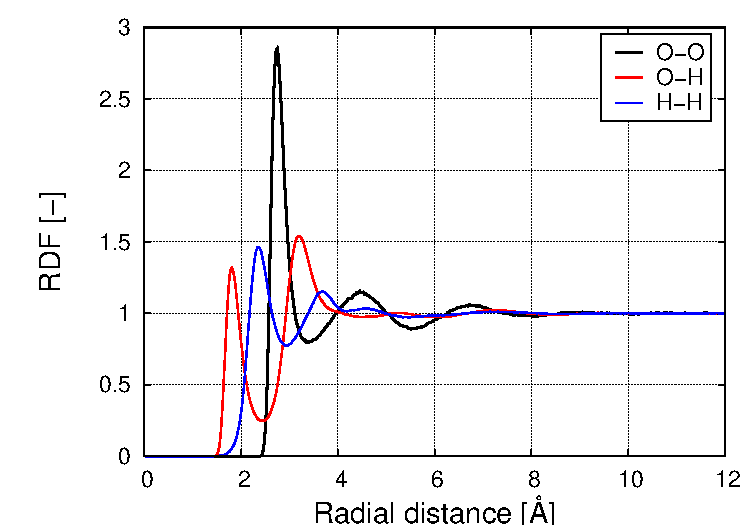
\includegraphics[width=7.5cm]{./Examples/RDFWater.pdf}
  \caption{The radial distribution function of water at 298K.}
  \label{Fig: RDF water}
\end{figure}

\subsection*{Example 9: Computing the radial distribution function of a methane/ethane-mixture}

The radial distribution function (RDF) is a good indication of the status of the fluid: solid, liquid or gas. RASPA
computes the RDF for all (pseudo-)atoms pairs, unless you specified `no' to the `PrintToPDB'-field of the `pseudo\_atoms' file.
For example, the $L$-atoms of water should not be printed to movie-files, and there would be little point generating
the RDF for interactions with these `dummy' interaction sites.
\begin{tiny}
\begin{verbatim}
     SimulationType                MolecularDynamics
     NumberOfCycles                1000000
     NumberOfInitializationCycles  10000
     NumberOfEquilibrationCycles   5000
     PrintEvery                    5000
     
     ContinueAfterCrash            no
     WriteBinaryRestartFileEvery   5000
     
     Ensemble                      NVT
     
     Forcefield                    GarciaPerez2006
     
     Box 0
     BoxLengths 24.0 24.0 24.0
     ComputeRDF yes
     WriteRDFEvery 10000
     RDFHistogramSize 300
     RDFRange 12.0
     ExternalTemperature 300.0
     
     Component 0 MoleculeName             methane
                 MoleculeDefinition       TraPPE
                 TranslationProbability   0.5
                 RotationProbability      0.5
                 ReinsertionProbability   1.0
                 CreateNumberOfMolecules  50
     
     Component 1 MoleculeName             ethane
                 MoleculeDefinition       TraPPE
                 TranslationProbability   0.5
                 RotationProbability      0.5
                 ReinsertionProbability   1.0
                 CreateNumberOfMolecules  50
\end{verbatim}
\end{tiny}

We used the NVT ensemble and therefore we have good temperature control
\begin{tiny}
\begin{verbatim}
     Temperature:             289.880 (avg.  299.641), Translational (avg.  299.641), Rotational (avg.      nan)
     Temperature Adsorbates:  289.880 (avg.  299.641), Translational (avg.  299.641), Rotational (avg.      nan)
\end{verbatim}
\end{tiny}

Shifted potentials are used and the relative energy conservation is 0.0000918675 (excellent).

\subsection*{Example 10: measuring bond/bend/dihedral angle distributions MD}

\begin{tiny}
\begin{verbatim}
     SimulationType                   MolecularDynamics
     NumberOfCycles                   10000000000
     NumberOfInitializationCycles     5000
     NumberOfEquilibrationCycles      10000
     PrintEvery                       10000
     RestartFile                      no
     
     Ensemble NVT
     
     ContinueAfterCrash               no
     WriteBinaryRestartFileEvery      5000
     
     Forcefield                       GarciaPerez2006
     
     Box 0
     BoxLengths 25 25 25
     ExternalTemperature 298.0
     ExternalPressure 0.0
     ComputeMoleculeProperties yes
     
     component 0 MoleculeName                     2-methylbutane
                 StartingBead                     0
                 FugacityCoefficient              1.0
                 MoleculeDefinition               TraPPE
                 TranslationProbability           1.0
                 RotationProbability              1.0
                 RegrowProbability                1.0
                 CBMCProbability                  1.0
                 CreateNumberOfMolecules          32
\end{verbatim}
\end{tiny}

\subsection*{Example 11: measuring bond/bend/dihedral angle distributions MC}


\begin{tiny}
\begin{verbatim}
     SimulationType                   MonteCarlo
     NumberOfCycles                   5000000
     NumberOfInitializationCycles     10000
     PrintEvery                       50000
     RestartFile                      no
     
     ContinueAfterCrash               no
     WriteBinaryRestartFileEvery      50000
     
     Forcefield                       GarciaPerez2006
     
     Box 0
     BoxLengths 25 25 25
     ExternalTemperature 298.0
     ExternalPressure 0.0
     ComputeMoleculeProperties yes
     
     component 0 MoleculeName                     2-methylbutane
                 StartingBead                     0
                 FugacityCoefficient              1.0
                 MoleculeDefinition               TraPPE
                 TranslationProbability           1.0
                 RotationProbability              1.0
                 RegrowProbability                1.0
                 CBMCProbability                  1.0
                 CreateNumberOfMolecules          32
\end{verbatim}
\end{tiny}

\begin{tiny}
\begin{verbatim}
\end{verbatim}
\end{tiny}

\begin{figure}[t]
  \centering
  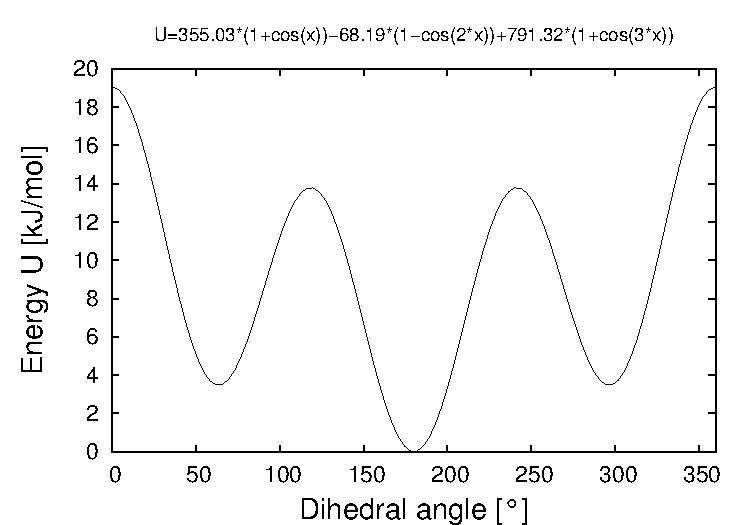
\includegraphics[width=7.5cm]{./Examples/ButaneUADihedral.pdf}
  \caption{The torsion potential for united atom linear alkanes X-CH$_2$-CH$_2$-X.}
  \label{Fig: Butane dihedral}
\end{figure}


\section{Non-basic examples}
\subsection*{Example 1: Adsorption of a binary CO$_2$/CH$_4$ (1:3) mixture in IRMOF-1}

Appreciable adsorption in MOF materials occurs at higher pressure than zeolites, usually in the range up to 10 bar. At these high pressures
absolute and excess adsorption are different, and excess adsorption eventually even goes down. This is due to the fact that excess adsorption is relative
to what would have been in the free pore volume at these conditions. So one can compress the outside fluid but eventually the pores are filled up. At that
maximum absolute loading the excess adsorption will go down.
\begin{tiny}
\begin{verbatim}
     SimulationType                MonteCarlo
     NumberOfCycles                50000
     NumberOfInitializationCycles  5000
     PrintEvery                    1000
     
     Forcefield                    Dubbeldam2007FlexibleIRMOF-1
     
     Framework 0
     FrameworkName IRMOF-1
     UnitCells 1 1 1
     HeliumVoidFraction 0.81
     ExternalTemperature 300.0
     ExternalPressure  10e5
     
     Component 0 MoleculeName               CO2
                 MoleculeDefinition         TraPPE
                 MolFraction                0.25
                 TranslationProbability     0.5
                 RegrowProbability          0.5
                 IdentityChangeProbability  1.0
                   NumberOfIdentityChanges  2
                   IdentityChangesList      0 1
                 SwapProbability            1.0
                 CreateNumberOfMolecules    0
     
     Component 1 MoleculeName               methane
                 MoleculeDefinition         TraPPE
                 MolFraction                0.75
                 TranslationProbability     0.5
                 RegrowProbability          0.5
                 IdentityChangeProbability  1.0
                   NumberOfIdentityChanges  2
                   IdentityChangesList      0 1
                 SwapProbability            1.0
                 CreateNumberOfMolecules    0
\end{verbatim}
\end{tiny}

To compute the excess adsorption the void fraction of a structure needs to be specified using `HeliumVoidFraction [real]'. RASPA automatically uses an
equation of state (default: Peng-Robinson) to compute the fugacities from the pressure and mol-fraction as is done here for a mixture of CO$_2$ and CH$_4$.
It also computes the amount of excess molecules from this equation of state.
\begin{tiny}
\begin{verbatim}
     Component 0 [CO2] (Adsorbate molecule)
     
             Critical temparure [K]: 304.128200
             Critical pressure [Pa]: 7377300.000000
             Acentric factor [-]: 0.223940
     
             RXMC partition factor [-]: 0.000000
     
             Fluid is a vapour
     
             MolFraction:           0.2500000000 [-]
             Compressibility:       0.9714389725 [-]
     
             Density of the bulk fluid phase:      18.1580726483 [kg/m^3]
     
             Binary mixture EOS parameters:  (0): 0.000000 (1): 0.000000
     
             Amount of excess molecules:       0.8675190741 [-]
     
             Conversion factor molecules/unit cell -> mol/kg:       0.1623747175 [-]
             Conversion factor molecules/unit cell -> gr/gr:       7.1442927209 [-]
             Conversion factor molecules/unit cell -> cm^3 STP/gr:       3.6394629804 [-]
             Conversion factor molecules/unit cell -> cm^3 STP/cm^3:       2.1592046669 [-]
             Conversion factor mol/kg -> cm^3 STP/gr:      22.4139757476 [-]
             Conversion factor mol/kg -> cm^3 STP/cm^3:      13.2976654244 [-]
     
             Partial pressure:    250000.00000000000000 [Pa]
                                    1875.00000000000000 [Torr]
                                       2.50000000000000 [bar]
                                       2.46730816679003 [atm]
     
             Fugacity coefficient:       0.9503504709 [-]
     
             Partial fugacity:    237587.61773457148229 [Pa]
                                    1781.90713300928610 [Torr]
                                       2.37587617734571 [bar]
                                       2.34480747825879 [atm]
     
     Component 1 [methane] (Adsorbate molecule)
     
             Critical temparure [K]: 190.564000
             Critical pressure [Pa]: 4599200.000000
             Acentric factor [-]: 0.011420
     
             RXMC partition factor [-]: 0.000000
     
             Fluid is a vapour
     
             MolFraction:           0.7500000000 [-]
             Compressibility:       0.9714389725 [-]
     
             Density of the bulk fluid phase:       6.6206386115 [kg/m^3]
     
             Binary mixture EOS parameters:  (0): 0.000000 (1): 0.000000
     
             Amount of excess molecules:       2.6025572224 [-]
     
             Conversion factor molecules/unit cell -> mol/kg:       0.1623747175 [-]
             Conversion factor molecules/unit cell -> gr/gr:       2.6048899107 [-]
             Conversion factor molecules/unit cell -> cm^3 STP/gr:       3.6394629804 [-]
             Conversion factor molecules/unit cell -> cm^3 STP/cm^3:       2.1592046669 [-]
             Conversion factor mol/kg -> cm^3 STP/gr:      22.4139757476 [-]
             Conversion factor mol/kg -> cm^3 STP/cm^3:      13.2976654244 [-]
     
             Partial pressure:    750000.00000000011642 [Pa]
                                    5625.00000000000091 [Torr]
                                       7.50000000000000 [bar]
                                       7.40192450037010 [atm]
     
             Fugacity coefficient:       0.9790119494 [-]
     
             Partial fugacity:    734258.96201743301935 [Pa]
                                    5506.94221513074717 [Torr]
                                       7.34258962017433 [bar]
                                       7.24657253409754 [atm]
\end{verbatim}
\end{tiny}
Also noteworthy is the use of the identity-change move for mixtures. A molecule of a certain type can be changed at the same position into a molecule of
another type. It is specified per component as a list of other components that are allowed for this move. The identity-change move is highly recommended
at high loadings.

At each `PrintEvery' steps the loadings are shown in a variety of units for both excess and absolute adsorption:
\begin{tiny}
\begin{verbatim}
     Loadings per component:
     ----------------------------------------------------------------------------------------------------------------------------------------------------------------------
     Component 0 (CO2), current number of integer/fractional/reaction molecules: 16/0/0 (avg.  12.68484), density:  67.81662 (avg.  53.76520) [kg/m^3]
             absolute adsorption:  16.00000 (avg.  12.68484) [mol/uc],   2.5979954802 (avg.   2.0596978259) [mol/kg], 114.3086835349 (avg.  90.6242327003) [mg/g]
                                   58.2314076859 (avg.  46.1660171161) [cm^3 STP/g],   34.5472746700 (avg.  27.3891725636) [cm^3 STP/cm^3]
             excess adsorption:    15.1324809259 (avg.  11.8173240923) [mol/uc],   2.4571323156 (avg.   1.9188346613) [mol/kg], 108.1108733282 (avg.  84.4264224936) [mg/g]
                                   55.0741041308 (avg.  43.0087135610) [cm^3 STP/g],   32.6741234365 (avg.  25.5160213301) [cm^3 STP/cm^3]
     Component 1 (methane), current number of integer/fractional/reaction molecules: 19/0/0 (avg.  19.21646), density:  29.36296 (avg.  29.69749) [kg/m^3]
             absolute adsorption:  19.00000 (avg.  19.21646) [mol/uc],   3.0851196328 (avg.   3.1202680711) [mol/kg],  49.4929083037 (avg.  50.0567757203) [mg/g]
                                   69.1497966270 (avg.  69.9376128722) [cm^3 STP/g],   41.0248886706 (avg.  41.4922808443) [cm^3 STP/cm^3]
             excess adsorption:    16.3974427776 (avg.  16.6139077477) [mol/uc],   2.6625301390 (avg.   2.6976785773) [mol/kg],  42.7135332529 (avg.  43.2774006695) [mg/g]
                                   59.6778859617 (avg.  60.4657022069) [cm^3 STP/g],   35.4054349701 (avg.  35.8728271438) [cm^3 STP/cm^3]
     ----------------------------------------------------------------------------------------------------------------------------------------------------------------------
\end{verbatim}
\end{tiny}
and at the end error bars are computed for all properties:
\begin{tiny}
\begin{verbatim}
     Component 0 [CO2]
     -------------------------------------------------------------
             Block[ 0] 12.55000           [-]
             Block[ 1] 12.79110           [-]
             Block[ 2] 12.75510           [-]
             Block[ 3] 12.73990           [-]
             Block[ 4] 12.58240           [-]
             ------------------------------------------------------------------------------
             Average                                     12.6837000000 +/-       0.1958132580 [-]
             Average loading absolute [molecules/unit cell]       12.6837000000 +/-       0.1958132580 [-]
             Average loading absolute [mol/kg framework]          2.0595122045 +/-       0.0317951224 [-]
             Average loading absolute [milligram/gram framework]         90.6160655845 +/-       1.3989472336 [-]
             Average loading absolute [cm^3 (STP)/gr framework]         46.1618566041 +/-       0.7126551035 [-]
             Average loading absolute [cm^3 (STP)/cm^3 framework]         27.3867042332 +/-       0.4228009005 [-]
     
             Average loading excess [molecules/unit cell]       11.8161809259 +/-       0.1958132580 [-]
             Average loading excess [mol/kg framework]          1.9186490399 +/-       0.0317951224 [-]
             Average loading excess [milligram/gram framework]         84.4182553778 +/-       1.3989472336 [-]
             Average loading excess [cm^3 (STP)/gr framework]         43.0045530490 +/-       0.7126551035 [-]
             Average loading excess [cm^3 (STP)/cm^3 framework]         25.5135529997 +/-       0.4228009005 [-]
     
     Component 1 [methane]
     -------------------------------------------------------------
             Block[ 0] 19.23430           [-]
             Block[ 1] 19.30250           [-]
             Block[ 2] 19.22250           [-]
             Block[ 3] 19.11980           [-]
             Block[ 4] 19.19560           [-]
             ------------------------------------------------------------------------------
             Average                                     19.2149400000 +/-       0.1184039594 [-]
             Average loading absolute [molecules/unit cell]       19.2149400000 +/-       0.1184039594 [-]
             Average loading absolute [mol/kg framework]          3.1200204545 +/-       0.0192258095 [-]
             Average loading absolute [milligram/gram framework]         50.0528033411 +/-       0.3084292792 [-]
             Average loading absolute [cm^3 (STP)/gr framework]         69.9320628000 +/-       0.4309268269 [-]
             Average loading absolute [cm^3 (STP)/cm^3 framework]         41.4889881217 +/-       0.2556583817 [-]
     
             Average loading excess [molecules/unit cell]       16.6123827776 +/-       0.1184039594 [-]
             Average loading excess [mol/kg framework]          2.6974309607 +/-       0.0192258095 [-]
             Average loading excess [milligram/gram framework]         43.2734282903 +/-       0.3084292792 [-]
             Average loading excess [cm^3 (STP)/gr framework]         60.4601521347 +/-       0.4309268269 [-]
             Average loading excess [cm^3 (STP)/cm^3 framework]         35.8695344212 +/-       0.2556583817 [-]
\end{verbatim}
\end{tiny}


\subsection*{Example 2: NPT Monte Carlo of propane}

The density of propane at 250K and 10 bar is about 559.53 kg/m$^3$ (NIST database). In this example the density is
computed using Monte Carlo in the NPT-ensemble. Given the pressure $P$, the temperature $T$, and the amount of molecules $N$,
the density is computed.

\begin{tiny}
\begin{verbatim}
     SimulationType                MonteCarlo
     NumberOfCycles                50000
     NumberOfInitializationCycles  10000
     PrintEvery                    1000
     RestartFile                   no
     
     Forcefield                    GarciaPerez2006
     
     Box 0
     BoxLengths 30 30 30
     ExternalTemperature 250.0
     ExternalPressure 1e6
     ComputeMolecularPressure yes
     
     VolumeChangeProbability       0.05
     
     Component 0 MoleculeName             propane
                 MoleculeDefinition       TraPPE
                 TranslationProbability   0.5
                 RotationProbability      0.5
                 RegrowProbability        0.5
                 CreateNumberOfMolecules  256
\end{verbatim}
\end{tiny}

The TraPPE model for propane gives for our simulation of 25000 cycles $568.2\pm 4.1$ kg/m$^3$.
The measured pressure is $9.75\pm2.2$ bar.


\subsection*{Example 3: NPT molecular dynamics of water}
A molecular dynamics simulation of water in the NPT-ensemble
(constant amount of particles $N$, constant average pressure $P$, and constant average temperature $T$).
Many water models are defined, but most are defined with simple Coulombic potentials using cutoffs of 9\AA.
None are optimized with the Ewald-summation except for the recalibrated Tip5p-Ew model.
Unfortunately, that model is defined using a cutoff always equal to half the box size, while
RASPA uses a fixed cutoff (default: 12 Angstrom). A fixed cutoff is more realistic, but requires the shortest
perpendicular width to be twice the cutoff, thus here larger than 24 \AA. All this results in having
to simulate more than 512 water molecules. The tip5p models use 5 fixed charges placed in the water geometry,
so for each step 2560 charge sites needs to be computed with Ewald. Conclusion: liquid water is computationally
expensive to compute when done properly.

In MD-NPT the average pressure 
$\left\langle P\right\rangle$ and average temperature $\left\langle T\right\rangle$ are imposed. The instantaneous
values, especially for the pressure, are different. RASPA uses the Nose-Hoover chain method, and NPT-MD methods of
Martyna and Tuckermann.

Several options are introduced here: "TimeStep [real]" to set the time step. For rigid molecules the time step can be a bit larger
because the high frequency movement is removed (the O-H is around 3000 cm$^{-1}$). The cutoff can be set with `CutOff [real]'.
The method to compute charge interactions is set with `ChargeMethod [Ewald$|$None]', although Ewald is the default. The precision can specified
using `EwaldPrecision [real]' from which the Ewald parameters $\kappa$ and the amount of wave vectors is inferred.
The initial positions of the water are read from file (`RestartFile yes'), the file is located in directory `RestartInitial/System[int]'.

The experimental density of water at 300K and 1 bar is about 996.56 kg/m$^3$ (NIST database).

\begin{tiny}
\begin{verbatim}
     SimulationType                MolecularDynamics
     NumberOfCycles                100000
     NumberOfInitializationCycles  0
     NumberOfEquilibrationCycles   1000
     PrintEvery                    100
     RestartFile                   yes

     Ensemble                      NPT
     TimeStep                      0.001

     ChargeMethod                  Ewald
     CutOff                        10.0
     Forcefield                    Tip5p-Ew
     EwaldPrecision                1e-6

     Box 0
     BoxLengths 24.83 24.83 24.83
     ExternalTemperature 300.0
     ExternalPressure 1.0e5
     ComputeMSD yes
     PrintMSDEvery 5000

     Component 0 MoleculeName             Tip5p
                 StartingBead             0
                 MoleculeDefinition       Water
                 TranslationProbability   1.0
                 RotationProbability      1.0
                 ReinsertionProbability   1.0
                 CreateNumberOfMolecules  0
\end{verbatim}
\end{tiny}

The output shows some details of intermediate status during the run: the time run, the current box and average box, etc.
The total linear momentum is conserved and zero (the center of mass movement of the system is removed at initialization).
For this relatively short run, the average pressure of 1.26 bar is already quite close to the applied 1 bar.
Also, the temperature of the water, and of the simulation cell (it is a degree of freedom and has therefore an associated temperature)
can also been seen to converge to the applied value of 300K. Energy conservation is adequate with a 0.001 ps time step.
\begin{tiny}
\begin{verbatim}
TODO
\end{verbatim}
\end{tiny}


\subsection*{Example 4: Adsorption of CO$_2$ in Na-LTA}

The Linde Type A structure LTA-4A has 96 aluminum per unit cell. A common 4A sample has 96 charge balancing sodium ions.
The ions are small enough to access the sodalite cages, but the bigger methane molecules are exclusively in the big $\alpha$-cages
and not in the sodalite cages. They need to be artificially blocked. 
Because the adsorption is dependent on the positions of the ions it is
important to start from the crystallographic positions and use \emph{only} translation for the ions. Reinsertion moves may transport the ions
to positions in the windows and this is especially important for diffusion (the next example).

\begin{tiny}
\begin{verbatim}
     SimulationType                   MonteCarlo
     NumberOfCycles                   25000
     NumberOfInitializationCycles     10000
     RestartFile                      no
     PrintEvery                       1000
     
     Forcefield                       GarciaPerez2006
     ModifyOxgensConnectedToAluminium yes
     
     Framework 0
     FrameworkName LTA4A
     RemoveAtomNumberCodeFromLabel yes
     UnitCells 1 1 1
     ExternalTemperature 298.0
     ExternalPressure 10000.0
     
     Component 0 MoleculeName                   sodium
                 MoleculeDefinition             TraPPE
                 TranslationProbability         1.0
                 RandomTranslationProbability   1.0
                 ExtraFrameworkMolecule         yes
                 CreateNumberOfMolecules        96
     
     Component 1 MoleculeName                   CO2
                 MoleculeDefinition             TraPPE
                 BlockPockets                   yes
                 BlockPocketsFilename           LTA
                 TranslationProbability         1.0
                 ReinsertionProbability         1.0
                 SwapProbability                1.0
                 ExtraFrameworkMolecule         no
                 CreateNumberOfMolecules        0
\end{verbatim}
\end{tiny}

\subsection*{Example 5: Diffusion of CO$_2$ in Na-LTA}

An example of molecular dynamics of an adsorbate (CO$_2$) diffusing through the pores of LTA 4A loaded with ions.
The ions are read from the restart-file. The mean-square displacement is computed during the run.

\begin{tiny}
\begin{verbatim}
     SimulationType                   MolecularDynamics
     NumberOfCycles                   250000
     NumberOfInitializationCycles     5000
     NumberOfEquilibrationCycles      10000
     PrintEvery                       5000
     RestartFile                      no
     
     Ensemble                         NVT
     
     Forcefield                       GarciaPerez2006
     ModifyOxgensConnectedToAluminium yes
     TimeStep                         0.0005
     
     Framework 0
     FrameworkName LTA4A
     RemoveAtomNumberCodeFromLabel yes
     UnitCells 1 1 1
     ExternalTemperature 600.0
     ComputeMSD yes
     PrintMSDEvery 5000
     
     component 0 MoleculeName             sodium
                 MoleculeDefinition       TraPPE
                 TranslationProbability   1.0
                 ReinsertionProbability   1.0
                 ExtraFrameworkMolecule   yes
                 CreateNumberOfMolecules  96
     
     component 1 MoleculeName             CO2
                 MoleculeDefinition       TraPPE
                 BlockPockets             yes
                 BlockPocketsFilename     LTA
                 TranslationProbability   1.0
                 RotationProbability      1.0
                 ReinsertionProbability   1.0
                 ExtraFrameworkMolecule   no
                 CreateNumberOfMolecules  64
\end{verbatim}
\end{tiny}

\subsection*{Example 6: Diffusion of benzene in rigid IRMOF-1}

Benzene (and aromatic molecules in general) are usually kept rigid. RASPA uses quaternions for the description of the
orientation of the molecules. The integration schemes of Martyna and Tuckermann are symplectic and conserve energy
very well. Even though the molecule is described as a center of mass and a orientation, the forces are still computed
atomically. In this example the diffusivity the mean-square displacement of benzene at 298K in IRMOF-1 is computed.
The forcefield is `FlexibleIRMOF-1' which is also perfectly suitable for rigid structures. It has been specifically
optimized for iso-reticular metal-organic frameworks.

\begin{tiny}
\begin{verbatim}
     SimulationType                MolecularDynamics
     NumberOfCycles                100000
     NumberOfEquilibrationCycles   10000
     NumberOfInitializationCycles  1000
     PrintEvery                    5000
     RestartFile                   no
     
     Ensemble                      NVT
     
     ChargeMethod                  Ewald
     CutOff                        12.0
     TimeStep                      0.0005
     Forcefield                    Dubbeldam2007FlexibleIRMOF-1
     EwaldPrecision                1e-6
     
     Framework 0
     FrameworkName IRMOF-1
     UnitCells 1 1 1
     ExternalTemperature 298.0
     
     Component 0 MoleculeName              benzene
                 StartingBead              0
                 MoleculeDefinition        TraPPE
                 IdealGasRosenbluthWeight  1.0
                 TranslationProbability    1.0
                 RotationProbability       1.0
                 RegrowProbability         1.0
                 CreateNumberOfMolecules   16
\end{verbatim}
\end{tiny}

\begin{figure}[t]
  \centering
  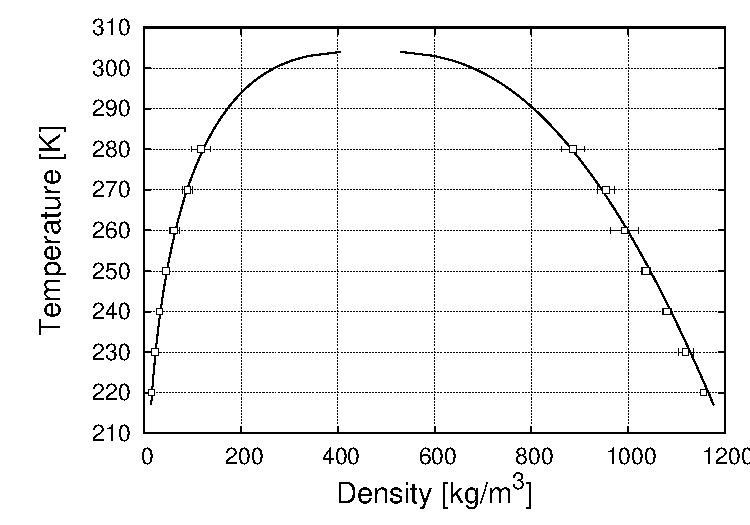
\includegraphics[width=7.5cm]{./Examples/GibbsCO2.pdf}
  \caption{Gibbs ensemble simulation of CO2 at 250K. Two simulation boxes are used: one for the gas-branch and one for the liquid branch. The simulation can
           only be conducted below a certain temperature because otherwise the boxes can swap between gas and liquid. At 250K, the boxes are initialized
           with an equal amount of molecules, but soon split into gas and liquid. The average densities are straightforward to measure. As shown, the
           TraPPE model for CO2 does a good job when compare to experimental data (NIST database).}
  \label{Fig: Gibbs CO2}
\end{figure}

\subsection*{Example 7: Gibbs ensemble simulation of CO$_2$}

The Gibbs ensemble is way of computing coexistence without interfaces. It is one the most used methods
to study vapor-liquid and liquid-liquid equilibria, it is not suitable for very dense systems. The 
conditions for coexistence of two or more phases I, II, \dots is that the pressure and temperature 
of all the phases must be equal, as well as the chemical potential of all the species. The Gibbs
ensemble example for the single component CO$_2$ is listed below. two boxes will be used, one will
correspond to the liquid phase, the other one to the gas phase. The `GibbsVolumeChange' move
changes the individual volume leaving the total volume in tact, the `GibbsSwap' move
swaps particles from one box to the other. One of the practical problems is to make sure both
boxes remain larger than twice the cutoff length. If not, the program will exit with an error message,
and the simulation should be restarted with a bigger volume. 
Note that RASPA uses orientational biased insertions for small rigid molecules like CO$_2$.
For this example about 10000-20000 cycles are needed to equilibrate properly.
\begin{tiny}
\begin{verbatim}
     SimulationType                MonteCarlo
     NumberOfCycles                25000
     NumberOfInitializationCycles  10000
     PrintEvery                    1000
     RestartFile                   no
     
     Forcefield                    TraPPE
     
     Box 0
     BoxLengths 30 30 30
     BoxAngles 90 90 90
     ExternalTemperature 240.0
     
     Box 1
     BoxLengths 30 30 30
     BoxAngles 90 90 90
     ExternalTemperature 240.0
     
     GibbsVolumeChangeProbability 0.1
     
     Component 0 MoleculeName             CO2
                 StartingBead             1
                 MoleculeDefinition       TraPPE
                 TranslationProbability   1.0
                 RotationProbability      1.0
                 ReinsertionProbability   1.0
                 GibbsSwapProbability     1.0
                 CreateNumberOfMolecules  150 150
\end{verbatim}
\end{tiny}

\subsection*{Example 8: Minimization of a flexible framework (fixed volume)}

Physically, energy minimization corresponds to an instantaneous freezing of the system; a static structure in 
which no atom feels a net force corresponds to a temperature of 0 K. In the early 1980's, energy minimization was 
about all one could afford to do and was dubbed `molecular mechanics.' Here, a difficult optimization problem:
a flexible framework, IRMOF-1, in a periodic unit cell, with many low energy modes.
The energy landscape of a framework is very complex. A true minimum is characterized by
all positive eigenvalues of the Hessian matrix (the matrix of second derivatives with respect to position). A
zero eigenvalue means that moving in the direction of the associated eigenvector does not result in a change in
energy. Likewise, a negative en positive eigenvalue means an decrease and increase in energy, respectively.
Most of the optimization time is spent on reaching a zero curvature structure, i.e. all positive eigenvalues.

\begin{tiny}
\begin{verbatim}
     SimulationType  Minimization
     NumberOfCycles  1
     RestartFile     no
     PrintEvery      1
     
     MaximumNumberOfMinimizationSteps 1000
     RMSGradientTolerance 1e-6
     MaxGradientTolerance 1e-6
     
     Ensemble        NVT
     
     Forcefield                                 Dubbeldam2007FlexibleIRMOF-1
     ChargeMethod                               Ewald
     EwaldPrecision                             1e-10
     InternalFrameworkLennardJonesInteractions  yes
     
     Framework 0
     FrameworkName IRMOF-1
     UnitCells 1 1 1
     ExternalTemperature 298.0
     Movies yes
     WriteMoviesEvery 1
     
     FlexibleFramework     yes
     FrameworkDefinitions  Dubbeldam2007FlexibleIRMOF-1
\end{verbatim}
\end{tiny}
The minimization needs 119 cycles to optimize IRMOF-1, the last steps are shown here. The convergence is very rapid (quadratic) near the minimum,
and the minimum energy can be reached up to arbitrary precision (the forces on all the atoms are $1\times10^{-8}$ K/\AA$^2$
or smaller). To compute spectra, frequencies and/or eigenmodes a high precision is needed.
\begin{tiny}
\begin{verbatim}
     Starting configuration:
           Box:      25.8320000000       0.0000000000       0.0000000000     Strain derivative:  129316.6369463501       0.0000000016       0.0000000015
                      0.0000000000      25.8320000000       0.0000000000                              0.0000000015  129316.6369463478       0.0000000016
                      0.0000000000       0.0000000000      25.8320000000                              0.0000000016       0.0000000015  129316.6369463608


     Beginning Baker minimization:
     -----------------------------
     Shifting parameter: -144554.0050033366 Lowest eigenvalue:   -1933.2972944159
     Iteration: 0 Energy: -4210346.0956447003 RMS gradient: 254.796  Max gradient: 16621.7 Number of negative eigenvalues: 30 Number of zero eigenvalues: 3
           Box:      25.8320000000       0.0000000000       0.0000000000     Strain derivative:  129316.6369463581       0.0000000016       0.0000000015
                      0.0000000000      25.8320000000       0.0000000000                              0.0000000016  129316.6369463568       0.0000000016
                      0.0000000000       0.0000000000      25.8320000000                              0.0000000015       0.0000000016  129316.6369463690
           Lengths:      25.8320000000      25.8320000000      25.8320000000, Angles:      90.0000000000      90.0000000000      90.0000000000

     Shifting parameter:  -54112.0433245863 Lowest eigenvalue:    -942.0341042027
     Iteration: 1 Energy: -4291359.2884553447 RMS gradient: 132.811  Max gradient: 9119.05 Number of negative eigenvalues: 30 Number of zero eigenvalues: 3
           Box:      25.8320000000       0.0000000000       0.0000000000     Strain derivative: -131739.2152028512       0.0000000004       0.0000000008
                      0.0000000000      25.8320000000       0.0000000000                              0.0000000004 -131739.2152028439       0.0000000010
                      0.0000000000       0.0000000000      25.8320000000                              0.0000000008       0.0000000011 -131739.2152028617
           Lengths:      25.8320000000      25.8320000000      25.8320000000, Angles:      90.0000000000      90.0000000000      90.0000000000

     Shifting parameter:   -6990.6349276451 Lowest eigenvalue:    -218.9092550725
     Iteration: 2 Energy: -4325503.0430874182 RMS gradient: 38.7491  Max gradient: 2721.14 Number of negative eigenvalues: 36 Number of zero eigenvalues: 3
           Box:      25.8320000000       0.0000000000       0.0000000000     Strain derivative: -282155.2863533634       0.0000000002       0.0000000007
                      0.0000000000      25.8320000000       0.0000000000                              0.0000000002 -282155.2863533496      -0.0000000021
                      0.0000000000       0.0000000000      25.8320000000                              0.0000000008      -0.0000000021 -282155.2863533603
           Lengths:      25.8320000000      25.8320000000      25.8320000000, Angles:      90.0000000000      90.0000000000      90.0000000000

     ..........................................................................

     Iteration: 117 Energy: -4331364.7259515934 RMS gradient: 0.00439145  Max gradient: 0.600384 Number of negative eigenvalues: 0 Number of zero eigenvalues: 3
           Box:      25.8320000000       0.0000000000       0.0000000000     Strain derivative:  -99169.3483007069       0.0011594244       0.0002624505
                      0.0000000000      25.8320000000       0.0000000000                              0.0011594245  -99108.1188463482      -0.0004447560
                      0.0000000000       0.0000000000      25.8320000000                              0.0002624506      -0.0004447560  -99128.0909746577
           Lengths:      25.8320000000      25.8320000000      25.8320000000, Angles:      90.0000000000      90.0000000000      90.0000000000

     Iteration: 118 Energy: -4331364.6575047411 RMS gradient: 7.06135e-05  Max gradient: 0.0204619 Number of negative eigenvalues: 0 Number of zero eigenvalues: 3
           Box:      25.8320000000       0.0000000000       0.0000000000     Strain derivative:  -99208.8822655176       0.0000019593      -0.0000031410
                      0.0000000000      25.8320000000       0.0000000000                              0.0000019594  -99184.4522480669      -0.0000004895
                      0.0000000000       0.0000000000      25.8320000000                             -0.0000031410      -0.0000004895  -99202.7818375186
           Lengths:      25.8320000000      25.8320000000      25.8320000000, Angles:      90.0000000000      90.0000000000      90.0000000000

     Iteration: 119 Energy: -4331364.6575191850 RMS gradient: 6.91407e-07  Max gradient: 8.83309e-05 Number of negative eigenvalues: 0 Number of zero eigenvalues: 3
           Box:      25.8320000000       0.0000000000       0.0000000000     Strain derivative:  -99195.5973070737       0.0000000048      -0.0000030267
                      0.0000000000      25.8320000000       0.0000000000                              0.0000000047  -99195.5991107764       0.0000000006
                      0.0000000000       0.0000000000      25.8320000000                             -0.0000030267       0.0000000006  -99195.6111130547
           Lengths:      25.8320000000      25.8320000000      25.8320000000, Angles:      90.0000000000      90.0000000000      90.0000000000

     SUCCES: RMS Gradient tolerance 0.0001 reached (6.91407e-07)
             Max Gradient tolerance 0.0001 reached (8.83309e-05)


\end{verbatim}
\end{tiny}
The shifting values are always lower than the lowest eigenvalues, both are negative and approach zero. At iteration 2, the lowest eigenvalues is closer
to zero, but still the amount of negative eigenvalues is 6 higher. Also increases in energy can occur. However, eventually the system is driven to
all positive eigenvalues (a true energy minimum without saddle points) and the lowest energy.
Note that minimization the structure in constant volume results in a finite (non-zero) stress. Minimization taking volume and shape changes into account
are usually easier, because the system is less constrained.
If one would like to also minimize the cell volume (isotropicly) use
\begin{tiny}
\begin{verbatim}
     Ensemble                         NPT
\end{verbatim}
\end{tiny}
or use for a change in cell-lengths and cell-angles
\begin{tiny}
\begin{verbatim}
     Ensemble                         NPTPR
\end{verbatim}
\end{tiny}


\section{Advanced examples}

\subsection*{Example 1: Adsorption of CO$_2$ in fully-flexible IRMOF-1 ($\mu VT$-ensemble)}

Flexibility in MOFs is more important than in zeolites. A very efficient move to change the whole framework (and actually
also the adsorbates) is have a short NVE MD-run and accept or reject the new configuration. This hybrid MD/MC move can be switched on using
`HybridMCMDMoveProbability  [real]', where [real] is the fraction of the move at each cycle.

\begin{tiny}
\begin{verbatim}
     SimulationType                MonteCarlo
     NumberOfCycles                50000
     NumberOfInitializationCycles  20000
     PrintEvery                    5000
     RestartFile                   no
     
     ChargeMethod                  Ewald
     CutOff                        12.0
     Forcefield                    Dubbeldam2007FlexibleIRMOF-1
     EwaldPrecision                1e-6
     
     Framework 0
     FrameworkName IRMOF-1
     UnitCells 1 1 1
     HeliumVoidFraction 0.801937
     FrameworkDefinitions Dubbeldam2007FlexibleIRMOF-1
     ExternalTemperature 233.0
     ExternalPressure  1e5
     
     FlexibleFramework yes
     
     HybridMCMDMoveProbability 1.0
     
     Component 0 MoleculeName              CO2
                 StartingBead              0
                 MoleculeDefinition        TraPPE
                 IdealGasRosenbluthWeight  1.0
                 TranslationProbability    1.0
                 RotationProbability       1.0
                 ReinsertionProbability    1.0
                 SwapProbability           1.0
                 CreateNumberOfMolecules   0
\end{verbatim}
\end{tiny}


\subsection*{Example 2: CO$_2$ adsorption in flexible IRMOF-1 (osmotic ensemble).}

Adsorption simulations using a flexible framework are very computationally demanding, the current example will 
probably run about a week. The equilibration is very important and it is best to start with a restart-file
obtained from the previous example at the same temperature. The directory `Restart' produced in the previous
example should be copied to `RestartInitial' and the option `RestartFile' should be set to `yes'.

\begin{tiny}
\begin{verbatim}
     SimulationType                MonteCarlo
     NumberOfCycles                50000
     NumberOfInitializationCycles  10000
     PrintEvery                    5000
     RestartFile                   no
     
     ChargeMethod                  Ewald
     CutOff                        12.0
     Forcefield                    Dubbeldam2007FlexibleIRMOF-1
     EwaldPrecision                1e-6
     TimeStep                      0.0005
     
     Framework 0
     FrameworkName IRMOF-1
     UnitCells 1 1 1
     HeliumVoidFraction 0.801937
     ExternalTemperature 298.0
     ExternalPressure 100e3
     
     FrameworkDefinitions Dubbeldam2007FlexibleIRMOF-1
     FlexibleFramework yes
     
     HybridNVEMoveProbability 1.0
       NumberOfHybridNVESteps 5
     VolumeChangeProbability  1.0
     
     Component 0 MoleculeName              CO2
                 StartingBead              0
                 MoleculeDefinition        TraPPE
                 IdealGasRosenbluthWeight  1.0
                 TranslationProbability    1.0
                 RotationProbability       1.0
                 ReinsertionProbability    1.0
                 SwapProbability           1.0
                 CreateNumberOfMolecules   0
\end{verbatim}
\end{tiny}

\subsection*{Example 3: NPT molecular dynamics of flexible IRMOF-1}

An NPT-ensemble simulation of a flexible framework IRMOF-1. This type of simulation can be used to compute the average
unit cell size at the desired temperature and pressure (and properties like the `volumetric expansion coefficient' etc).
The equilibration, although slow, is very much faster than Monte Carlo. The example show the code for flexible
IRMOF-1 at 298K and 1 atm.

\begin{tiny}
\begin{verbatim}
     SimulationType               MolecularDynamics
     NumberOfCycles               500000
     NumberOfEquilibrationCycles  5000
     PrintEvery                   5000
     RestartFile                  no
     
     Ensemble                     NPT
     
     Forcefield                   Dubbeldam2007FlexibleIRMOF-1
     CutOff                       12.0
     
     Framework 0
     FrameworkName IRMOF-1
     UnitCells 1 1 1
     ExternalTemperature 298.0
     ExternalPressure 101325.0
     
     FlexibleFramework yes
     FrameworkDefinitions Dubbeldam2007FlexibleIRMOF-1
\end{verbatim}
\end{tiny}


\subsection*{Example 4: Benzene diffusion in flexible IRMOF-10}

Molecules with a phenyl-ring are usually quite rigid. In Monte Carlo rigid units are not a problem, because the MC moves can be developed in such a way that the
constraints remain satisfied, i.e. translation and rotation of the whole rigid unit. In molecular dynamics, there are two general approaches. The first is to integrate
the molecules atomically and afterwards satisfy the constraints iteratively using for example the shake algorithm. For bigger molecules complications arise, convergence
becomes more difficult, and for a planar molecule like benzene additional sites above the molecule are needed. Therefore, the second approach has become more popular. 
Using quaternions (or Euler angles) one can describe the configurations of the molecule as a center-of-mass position and an orientation. The translation and rotation
are integrated and when the forces are needed the atoms positions are computed from the com position and the orientation. The forces are then summed to the center of mass
and the torque is computed. Miller et al. have developed an integration algorithm for rigid units (using quaternions) that is symplectic.

All these techniques are combined in the example of diffusion of benzene in IRMOF-10. The integration is performed in the NVT ensemble using the Nose-Hoover thermostats.
Three separate NH chains are operating on (i) the translation, (ii) the rotation of the molecules, and (iii) on the framework.

\begin{tiny}
\begin{verbatim}
     SimulationType                MolecularDynamics
     NumberOfCycles                1000000
     NumberOfEquilibrationCycles   10000
     NumberOfInitializationCycles  100
     PrintEvery                    5000
     RestartFile                   no
     
     Ensemble                      NVT
     
     ChargeMethod                  Ewald
     CutOff                        12.0
     TimeStep                      0.0005
     Forcefield                    Dubbeldam2007FlexibleIRMOF-10
     EwaldPrecision                1e-6
     
     Framework 0
     FrameworkName IRMOF-10
     UnitCells 1 1 1
     ExternalTemperature 298.0
     Movies no
     WriteMoviesEvery 1000
     
     FrameworkDefinitions Dubbeldam2007FlexibleIRMOF-10
     FlexibleFramework yes
     
     Component 0 MoleculeName              benzene
                 StartingBead              0
                 MoleculeDefinition        TraPPE
                 IdealGasRosenbluthWeight  1.0
                 TranslationProbability    1.0
                 RotationProbability       1.0
                 ReinsertionProbability    1.0
                 CreateNumberOfMolecules   16
\end{verbatim}
\end{tiny}

\subsection*{Example 5: Continuous Fractional Component Monte Carlo}

A mixture simulation of CO2 and N2 in DMOF. The charges of DMOF are listed in the CIF-File using the `\_atom\_site\_charge' keyword,
and RASPA makes use of these usinf the keyword `UseChargesFromCIFFile yes'.
The CFCMC method is switched on by using `CFSwapLambdaProbability' (instead of `SwapProbability') to swap molecules in and out of the system at a fixed fugacity.
The biasing factors are measured using Wang-Landau sampling during `NumberOfEquilibrationCycles 50000'.

\begin{tiny}
\begin{verbatim}
     SimulationType                MonteCarlo
     NumberOfCycles                250000
     NumberOfEquilibrationCycles   50000
     PrintEvery                    5000
     RestartFile                   no
     
     ContinueAfterCrash no
     WriteBinaryRestartFileEvery 5000
     
     ChargeMethod                  Ewald
     Forcefield                    local
     CutOffVDW                     11.5
     RemoveAtomNumberCodeFromLabel no
     
     Framework             0
     FrameworkName         DMOF
     UseChargesFromCIFFile yes
     UnitCells             1 1 1
     HeliumVoidFraction    0.614
     ExternalTemperature   300
     ExternalPressure      1e5
     
     Component 0 MoleculeName              CO2
                 StartingBead              0
                 MoleculeDefinition        TraPPE
                 IdealGasRosenbluthWeight  1
                 FugacityCoefficient       1.0
                 TranslationProbability    1.0
                 RotationProbability       1.0
                 ReinsertionProbability    1.0
                 CBMCProbability           0.0
                 IdentityChangeProbability 1.0
                   NumberOfIdentityChanges 2
                   IdentityChangesList     0 1
                 SwapProbability           0.0
                 CFSwapLambdaProbability   1.0
                 CreateNumberOfMolecules   0
     
     Component 1 MoleculeName              N2
                 StartingBead              0
                 MoleculeDefinition        TraPPE
                 IdealGasRosenbluthWeight  1
                 FugacityCoefficient       1.0
                 TranslationProbability    1.0
                 RotationProbability       1.0
                 ReinsertionProbability    1.0
                 CBMCProbability           0.0
                 IdentityChangeProbability 1.0
                   NumberOfIdentityChanges 2
                   IdentityChangesList     0 1
                 SwapProbability           0.0
                 CFSwapLambdaProbability   1.0
                 CreateNumberOfMolecules   0
\end{verbatim}
\end{tiny}

The performance of the CFCMC is written at the end of the output file (after the run has finished).
The biasing factors have lead to relatively flat distribution of Lambda. The efficiency of insertion is
much higher (sometimes dramatically higher) than using conventional MC or even CBMC.

\begin{tiny}
\begin{verbatim}
     Performance of the CFMC swap lambda move:
     =========================================
     Component [CO2] total tried: 609238.000000 constant-lambda accepted: 378163.000000 (62.071473 [%])
                    total tried: 306306.000000 insert-lambda accepted: 75081.000000 (24.511763 [%])
                    total tried: 303052.000000 remove-lambda accepted: 75005.000000 (24.749878 [%])
     
             Lambda probabilities:
             ---------------------
             Lambda [ 0.000000 - 0.047619 ]:       4.6286053786 (biasing factor:       0.0000000000)
             Lambda [ 0.047619 - 0.095238 ]:       4.8557520294 (biasing factor:      -0.0382812500)
             Lambda [ 0.095238 - 0.142857 ]:       4.5367783909 (biasing factor:      -0.1300000000)
             Lambda [ 0.142857 - 0.190476 ]:       4.8916129710 (biasing factor:      -0.1393750000)
             Lambda [ 0.190476 - 0.238095 ]:       5.0546694721 (biasing factor:      -0.1734375000)
             Lambda [ 0.238095 - 0.285714 ]:       4.5641049207 (biasing factor:      -0.3854687500)
             Lambda [ 0.285714 - 0.333333 ]:       4.7402092244 (biasing factor:      -0.4912500000)
             Lambda [ 0.333333 - 0.380952 ]:       4.7959290856 (biasing factor:      -0.6443750000)
             Lambda [ 0.380952 - 0.428571 ]:       4.8145570804 (biasing factor:      -0.8160937500)
             Lambda [ 0.428571 - 0.476190 ]:       4.5662385237 (biasing factor:      -1.0582812500)
             Lambda [ 0.476190 - 0.523810 ]:       4.7369267583 (biasing factor:      -1.2257812500)
             Lambda [ 0.523810 - 0.571429 ]:       4.6820275136 (biasing factor:      -1.4496875000)
             Lambda [ 0.571429 - 0.619048 ]:       4.7426710739 (biasing factor:      -1.6581250000)
             Lambda [ 0.619048 - 0.666667 ]:       4.8326106437 (biasing factor:      -1.8906250000)
             Lambda [ 0.666667 - 0.714286 ]:       4.5595094683 (biasing factor:      -2.1996875000)
             Lambda [ 0.714286 - 0.761905 ]:       4.7041020978 (biasing factor:      -2.4212500000)
             Lambda [ 0.761905 - 0.809524 ]:       4.9031016022 (biasing factor:      -2.6934375000)
             Lambda [ 0.809524 - 0.857143 ]:       4.7744289330 (biasing factor:      -3.0331250000)
             Lambda [ 0.857143 - 0.904762 ]:       4.8093051348 (biasing factor:      -3.3956250000)
             Lambda [ 0.904762 - 0.952381 ]:       4.7984729968 (biasing factor:      -3.8495312500)
             Lambda [ 0.952381 - 1.000000 ]:       5.0083867008 (biasing factor:      -4.3439062500)
     
     Component [N2] total tried: 609131.000000 constant-lambda accepted: 416943.000000 (68.448823 [%])
                    total tried: 308180.000000 insert-lambda accepted: 94913.000000 (30.797910 [%])
                    total tried: 303197.000000 remove-lambda accepted: 94992.000000 (31.330125 [%])
             Lambda probabilities:
             Lambda [ 0.000000 - 0.047619 ]:       4.5778479125 (biasing factor:       0.0000000000)
             Lambda [ 0.047619 - 0.095238 ]:       4.6920626493 (biasing factor:       0.0130468750)
             Lambda [ 0.095238 - 0.142857 ]:       4.5589213672 (biasing factor:       0.0173437500)
             Lambda [ 0.142857 - 0.190476 ]:       4.5372090965 (biasing factor:       0.0282812500)
             Lambda [ 0.190476 - 0.238095 ]:       4.7957080167 (biasing factor:       0.0900781250)
             Lambda [ 0.238095 - 0.285714 ]:       4.8075063826 (biasing factor:       0.0614062500)
             Lambda [ 0.285714 - 0.333333 ]:       4.8118488367 (biasing factor:       0.0159375000)
             Lambda [ 0.333333 - 0.380952 ]:       4.8087353790 (biasing factor:      -0.0679687500)
             Lambda [ 0.380952 - 0.428571 ]:       4.7098421313 (biasing factor:      -0.1794531250)
             Lambda [ 0.428571 - 0.476190 ]:       4.8561746420 (biasing factor:      -0.2247656250)
             Lambda [ 0.476190 - 0.523810 ]:       4.9319627565 (biasing factor:      -0.3290625000)
             Lambda [ 0.523810 - 0.571429 ]:       4.7724390172 (biasing factor:      -0.4631250000)
             Lambda [ 0.571429 - 0.619048 ]:       4.7635083097 (biasing factor:      -0.5971093750)
             Lambda [ 0.619048 - 0.666667 ]:       4.5849760919 (biasing factor:      -0.7748437500)
             Lambda [ 0.666667 - 0.714286 ]:       4.8377396953 (biasing factor:      -0.8583593750)
             Lambda [ 0.714286 - 0.761905 ]:       4.8470800683 (biasing factor:      -0.9987500000)
             Lambda [ 0.761905 - 0.809524 ]:       4.7574452605 (biasing factor:      -1.1678125000)
             Lambda [ 0.809524 - 0.857143 ]:       4.8400338220 (biasing factor:      -1.3005468750)
             Lambda [ 0.857143 - 0.904762 ]:       4.8914058736 (biasing factor:      -1.4714062500)
             Lambda [ 0.904762 - 0.952381 ]:       4.9600658087 (biasing factor:      -1.6489843750)
             Lambda [ 0.952381 - 1.000000 ]:       4.6574868825 (biasing factor:      -1.8750000000)
\end{verbatim}
\end{tiny}

The computed loadings are averages of integer molecules.

\subsection*{Example 6: Reaction ensemble}

As an example, the industrially important propene metathesis is described by three equilibrium reactions
\begin{itemize}
\item{2 C$_3$H$_6$ $\leftrightarrow$ C$_2$H$_4$ + trans-C$_4$H$_8$}
\item{2 C$_3$H$_6$ $\leftrightarrow$ C$_2$H$_4$ + cis-C$_4$H$_8$}
\item{cis-C$_4$H$_8$ $\leftrightarrow$ trans-C$_4$H$_8$}
\end{itemize}
Only two reactions are independent and need to be included. In addition to the MC moves associated with
simulating a chosen ensemble, also ``reaction'' moves are performed:
\begin{enumerate}
\item{randomly choose a reaction,}
\item{randomly choose whether to do a forward or backward reaction (this determines the ``reactant'' and ``product'' molecule types),}
\item{randomly select the reactant molecules and remove them from the system},
\item{insert the product molecules at random positions},
\item{accept or reject the reaction step with the appropriate acceptance probability.}
\end{enumerate}

\begin{tiny}
\begin{verbatim}
     SimulationType                MC
     NumberOfCycles                100000
     NumberOfInitializationCycles  0
     NumberOfEquilibrationCycles   25000
     RestartFile                   no
     PrintEvery                    1000
     
     ContinueAfterCrash no
     WriteBinaryRestartFileEvery 500
     
     ChargeMethod                  none
     Forcefield                    local
     CutOff                        12.0
     EwaldPrecision                1e-6
     
     Box 0
     BoxLengths 150 150 150
     ExternalTemperature 450.0
     ExternalPressure 101300.0
     CutOff  14.0
     ComputeNumberOfMoleculesHistogram yes
     WriteNumberOfMoleculesHistogramEvery 5000
     
     Reaction 2 0 0 0 0 1 0 1
     Reaction 0 0 0 1 0 0 1 0
     
     ProbabilityCFCRXMCLambdaChangeMove 1.0
     VolumeChangeProbability            0.1
     
     Component 0 MoleculeName             propene
                 MoleculeDefinition       TraPPE
                 PartitionFunction        6.977909e37
                 TranslationProbability   35.0
                 RotationProbability      53.9
                 ReinsertionProbability   10.0
                 ExtraFrameworkMolecule   no
                 CreateNumberOfMolecules  400
     
     Component 1 MoleculeName             ethene
                 MoleculeDefinition       TraPPE
                 PartitionFunction        4.217717e35
                 TranslationProbability   35.0
                 RotationProbability      53.9
                 ReinsertionProbability   10.0
                 ExtraFrameworkMolecule   no
                 CreateNumberOfMolecules  0
     
     Component 2 MoleculeName             cis-2-butene
                 MoleculeDefinition       TraPPE
                 PartitionFunction        4.666103e38
                 TranslationProbability   35.0
                 RotationProbability      53.9
                 ReinsertionProbability   10.0
                 ExtraFrameworkMolecule   no
                 CreateNumberOfMolecules  0
     
     Component 3 MoleculeName             trans-2-butene
                 MoleculeDefinition       TraPPE
                 PartitionFunction        7.355798e38
                 TranslationProbability   35.0
                 RotationProbability      53.9
                 ReinsertionProbability   10.0
                 ExtraFrameworkMolecule   no
                 CreateNumberOfMolecules  0
\end{verbatim}
\end{tiny}
Reactions are given as a list of stoichometries for the reactants and then the products, so there should two times the number-of-components integer numbers.

In the output you will see for each PrintEvery the number of integer, fractional, and reaction molecules.
For each reaction the biasing factors are listed.
\begin{tiny}
\begin{verbatim}
     Reactions:
     ----------------------------------------------------------------------------------------------------------------------------------------------------
     Reaction 0, current Lambda:       0.7426373180, maximum Lambda-change:       1.0000000000
             Fractional molecules:  338 (ethene) 389 (trans-2-butene) <--> 375 (propene) 291 (propene)
             Biasing Factors: 0.000000 0.011875 0.040000 0.024375 0.014375 0.036250 -0.039375 0.008125 0.019375 -0.013750
                              0.002500 -0.011875 0.052500 0.013750 0.000625 -0.021250 -0.017500 -0.016250 -0.063125 -0.034375
                              -0.060625
     Reaction 1, current Lambda:       0.6428890080, maximum Lambda-change:       1.0000000000
             Fractional molecules:  236 (cis-2-butene) <--> 243 (trans-2-butene)
             Biasing Factors: 0.000000 0.014375 -0.023125 0.027500 -0.007500 0.038750 -0.004375 0.062500 0.016250 0.019375
                              -0.020000 0.065625 0.074375 0.006250 0.023125 0.054375 0.017500 0.038750 0.005000 0.037500
                              -0.054375
     
     Amount of molecules per component:
     ---------------------------------------------------------------------------------------------------------------------------------------------------------------
     Component 0 (propene), current number of integer/fractional/reaction molecules: 240/0/2 (average 243.80499), density:   0.70559 (average   0.68615) kg/m^3]
     Component 1 (ethene), current number of integer/fractional/reaction molecules: 80/0/1 (average  78.09750), density:   0.15680 (average   0.14652) kg/m^3]
     Component 2 (cis-2-butene), current number of integer/fractional/reaction molecules: 32/0/1 (average  30.20586), density:   0.12544 (average   0.11333) kg/m^3]
     Component 3 (trans-2-butene), current number of integer/fractional/reaction molecules: 48/0/2 (average  47.89165), density:   0.18816 (average   0.17970) kg/m^3]
     -----------------------------------------------------------------------------------------------------------------------------------------------------------------
\end{verbatim}
\end{tiny}

At the end of the output, after the run has finished, the statistics of the RXMC are printed:
\begin{tiny}
\begin{verbatim}
     Performance of the Reaction MC lambda move:
     ===========================================
     Reaction [0] total tried: 524722.000000 constant-lambda accepted: 508906.000000 (96.985832 [%])
                    total tried: 242207.000000 forward-reaction accepted: 219761.000000 (90.732720 [%])
                    total tried: 247919.000000 backward-reaction accepted: 219688.000000 (88.612813 [%])
     
     Reaction [1] total tried: 524439.000000 constant-lambda accepted: 509833.000000 (97.214929 [%])
                    total tried: 244749.000000 forward-reaction accepted: 219887.000000 (89.841838 [%])
                    total tried: 245258.000000 backward-reaction accepted: 219863.000000 (89.645598 [%])
\end{verbatim}
\end{tiny}
\section{Auxiliary examples}

\subsection*{Example 1: Computing the ideal gas Rosenbluth weight of a molecule}

To compare simulation values to experiments a reference state should be chosen. A convenient reference state
is the ideal gas. The reference Rosenbluth value can be computed from a simulation of a single chain at the
desired temperature. Note that for Rosenbluth weights several chains can be computed simultaneously, since
they are computed from Widom insertions where the molecule is never actually inserted in the system.

\begin{tiny}
\begin{verbatim}
     SimulationType        MonteCarlo
     NumberOfCycles        25000
     PrintEvery            1000
     PrintPropertiesEvery  1000
     
     Forcefield            GarciaPerez2006
     
     Box 0
     BoxLengths 30 30 30
     ExternalTemperature 573.0
     
     Component 0 MoleculeName              C5
                 MoleculeDefinition        TraPPE
                 WidomProbability          1.0
                 CreateNumberOfMolecules   0
     
     Component 1 MoleculeName              C6
                 MoleculeDefinition        TraPPE
                 WidomProbability          1.0
                 CreateNumberOfMolecules   0
     
     Component 2 MoleculeName              C7
                 MoleculeDefinition        TraPPE
                 WidomProbability          1.0
                 CreateNumberOfMolecules   0
     
     Component 3 MoleculeName              C8
                 MoleculeDefinition        TraPPE
                 WidomProbability          1.0
                 CreateNumberOfMolecules   0
     
     Component 4 MoleculeName              C9
                 MoleculeDefinition        TraPPE
                 WidomProbability          1.0
                 CreateNumberOfMolecules   0
\end{verbatim}
\end{tiny}
\noindent
The output contains 
\begin{tiny}
\begin{verbatim}
     Average Widom Rosenbluth factor:
     ================================
             [C5] Average Widom:   0.0668555 +/- 0.000131 [-]
             [C6] Average Widom:   0.0175062 +/- 0.000067 [-]
             [C7] Average Widom:   0.00462547 +/- 0.000010 [-]
             [C8] Average Widom:   0.00122842 +/- 0.000005 [-]
             [C9] Average Widom:   0.000328228 +/- 0.000001 [-]
\end{verbatim}
\end{tiny}
which is printed every `PrintPropertiesEvery' cycles. The `Rosenbluth factor new' are the values of interest.
The average and error estimated from block averages is printed at the end
of the simulation.


\subsection*{Example 2: Computing the helium void-fraction of a structure (pore volume)}

The void fraction is the empty space of a structure divided by the total volume. In experiment it
is measured using helium, because helium does (almost) not adsorb. It would be consistent to also
measure this fraction using helium at room temperature. In practice it is easily computed from
Widom particle insertion as the void fraction corresponds to the new Rosenbluth weight.
\begin{tiny}
\begin{verbatim}
     SimulationType        MonteCarlo
     NumberOfCycles        500000
     PrintEvery            1000
     PrintPropertiesEvery  1000
     
     Forcefield            GenericMOFs
     
     Framework 0
     FrameworkName IRMOF-1
     UnitCells 1 1 1
     ExternalTemperature 298.0
     
     
     Component 0 MoleculeName             helium
                 MoleculeDefinition       TraPPE
                 WidomProbability         1.0
                 CreateNumberOfMolecules  0
\end{verbatim}
\end{tiny}

The Rosenbluth weight, and therefore the helium void fraction of IRMOF-1 is approximately 0.80.
The pore volume is the void fraction times the unit cell volume. Note that the values dependent
slightly on the cutoff, and shifted vs. truncated potentials.
\begin{tiny}
\begin{verbatim}
     Average Widom Rosenbluth factor:
     ================================
             Block[ 0] 0.803749 [-]
             Block[ 1] 0.803741 [-]
             Block[ 2] 0.803497 [-]
             Block[ 3] 0.803818 [-]
             Block[ 4] 0.803536 [-]
             ------------------------------------------------------------------------------
             [helium] Average Widom:   0.803668 +/- 0.000255 [-]
\end{verbatim}
\end{tiny}

\subsection*{Example 3: Computing the surface area of IRMOF-1}

The geometric surface area can easily be computed by `rolling an atom over the surface' and measure the surface. In practice,
for each framework atom points are generate on a sphere around the framework atom, and the amount of overlap with other framework
atoms is determined. The fraction of overlap is multiplied times the area of the sphere. The summation over all framework atoms
gives the geometric surface area. This example shows how to compute the surface area of IRMOF-1. `SurfaceAreaSamplingPointsPerShere'
is the amount of points generated on sphere at a distance dependent on the mixing rule, the probe-atom and the current framework atom type.
The more points the higher the accuracy. The simulation usually takes between 5 and 30 minutes.

In this example the structure is probed with hydrogen using the second bead (`H\_com' with $\sigma=2.958$ \AA). The option
`SurfaceAreaProbeDistance Sigma' sets the overlap criteria to $\sigma$ instead of the default $\sigma^{1/6}$.

\begin{tiny}
\begin{verbatim}
     SimulationType        MonteCarlo
     NumberOfCycles        10000
     PrintEvery            100
     PrintPropertiesEvery  100
     
     Forcefield Dubbeldam2007FlexibleIRMOF-1
     CutOff 12.8
     
     Framework 0
     FrameworkName IRMOF-1
     UnitCells 1 1 1
     SurfaceAreaProbeDistance Sigma
     
     Component 0 MoleculeName             hydrogen
                 StartingBead             1
                 MoleculeDefinition       TraPPE
                 SurfaceAreaProbability   1.0
                 CreateNumberOfMolecules  0
\end{verbatim}
\end{tiny}
The area depends on the probe atom and on whether the well-depth at $2^{1/6}\sigma$ ($\approx 1.12246\sigma$)
is used (`SurfaceAreaProbeDistance Minimum')
\begin{tiny}
\begin{verbatim}
     Surface area: 2082.509853 [m^2/cm^3]
     Surface area: 3510.189484 [m^2/g]
\end{verbatim}
\end{tiny}
or $\sigma$ is used as the distance criteria (`SurfaceAreaProbeDistance Sigma'):
\begin{tiny}
\begin{verbatim}
     Surface area: 2266.243128 [m^2/cm^3]
     Surface area: 3819.882429 [m^2/g]
\end{verbatim}
\end{tiny}


\subsection*{Example 4: Powder diffraction pattern}

Powder diffraction is a scientific technique using X-Ray or neutron diffraction on powder or microcrystalline samples
for structural characterization of materials.
The most widespread use of powder diffraction is in the identification and characterization of crystalline solids,
each of which produces a distinctive diffraction pattern. Both the positions (corresponding to lattice spacings) and
the relative intensity of the lines are indicative of a particular phase and material, providing a "fingerprint" for comparison.
The database of IZA for zeolite has the option to generate the powder diffraction pattern:
\begin{tiny}
\begin{verbatim}
     http://izasc.ethz.ch/fmi/xsl/IZA-SC/xrd.xsl
\end{verbatim}
\end{tiny}

Here, an example of the powder diffraction pattern for the TON-type zeolite. Only one unit cell is sufficient for the computation
(interactions are not needed in the computation, just the position and types of the atoms and the shape and size of the unit cell).
The diffraction pattern usually takes a few seconds of computation, and the result is written to `PowderDiffraction/System[0]/'. It contains
two files: `PeakInformation.dat' and `Spectrum.dat'.
\begin{tiny}
\begin{verbatim}
     SimulationType  MonteCarlo
     NumberOfCycles  0

     Forcefield      ElenaSodiumCalcium

     Framework 0
     FrameworkName TON
     UnitCells 1 1 1

     ComputePowderDiffractionPattern yes
     DiffractionType Xray
     DiffractionRadiationType Copper
     WaveLengthType single
     TwoThetaMin 1
     TwoThetaMax 50
     TwoThetaStep 0.02
     PeakShape PseudoVoigt
     PeakWidthModifierU 0.005
\end{verbatim}
\end{tiny}

The first elements of the file `PeakInformation.dat' look like:
\begin{tiny}
\begin{verbatim}
     # 2-theta   d         h  k  l  Mult Lp          Scat. Factor    Intensity
       8.15213   0.09220 [ 1, 1, 0]    4 392.85927   19014.2044440544   100.000000
      10.15550   0.11481 [ 0,-2, 0]    2 252.33302   12381.2641234081    20.911920
      12.77464   0.14431 [ 2, 0, 0]    2 158.63285   19714.5657150741    20.933178
      16.34589   0.18441 [ 2, 2, 0]    4  96.01738    6730.9888808237     8.651941
      16.55216   0.18672 [-1,-3, 0]    4  93.58434     739.8429009358     0.926889
      19.42690   0.21886 [-1,-1,-1]    4  67.33674    3040.0925085839     2.740461
      .......................................
\end{verbatim}
\end{tiny}
So, the elements are the angle $2\theta$, the $d$-spacing, the Miller indices $h$,$k$, and $l$, the multiplicity,
the Lorentz-Polarization factor, the scattering factor (including anomalous scattering), and the relative intensity (where
the largest intensity is set to 100).
The second file `Spectrum.dat' can be plotted using gnuplot, the first column is $2\theta$, the second column the intensity.
The shape of the peaks can be influenced with `PeakShape', and the peak width modifiers `PeakWidthModifierU',
`PeakWidthModifierV', and `PeakWidthModifierW'.

\subsection*{Example 5: Making and using `grids'}

For rigid frameworks one can precompute the energy-grid, because the potential energy field induces by the framework does
not evolve in time. For each of the pseudo atoms one can generate a 3D grid where the spacing can be defined. In the example
the grid points are 0.1 \AA\ spaced apart (a=b=c=25.832\AA, $258\times258\times258=17173512$ points). 
A shorter distance results in more points, more accuracy, but also a bigger
grid (more memory is needed). Note that RASPA can handle a `mixture' of grids and fully computed interactions.
The table stores $U,\frac{\partial U}{\partial x}$, $\frac{\partial U}{\partial y}$, $\frac{\partial U}{\partial z}$,
$\frac{\partial^2 U}{\partial x\partial y}$, $\frac{\partial^2 U}{\partial x\partial z}$, $\frac{\partial^2 U}{\partial y\partial z}$,
and $\frac{\partial^3 U}{\partial x\partial y \partial z}$ at each grid point. The interpolation can handle non-orthorhombic cells
and can also be used for molecular dynamics (i.e. the force interpolation is consistent with the energy interpolation).

\begin{tiny}
\begin{verbatim}
     SimulationType  MakeGrid

     Forcefield      FlexibleIRMOF-1

     Framework 0
     FrameworkName IRMOF-1
     UnitCells 1 1 1

     NumberOfGrids 2
     GridTypes C_co2 O_co2
     SpacingVDWGrid 0.1
     SpacingCoulombGrid 0.1
\end{verbatim}
\end{tiny}
\noindent The grids are stored in `/share/raspa/grids/FlexibleIRMOF-1/IRMOF-1/0.100000' and the names are
`IRMOF-1\_C\_co2\_shifted.grid', `IRMOF-1\_O\_co2\_shifted.grid', and `IRMOF-1\_Electrostatics\_Ewald.grid'.
The last grid is the real part of the Ewald summation, i.e. erfc(r)/r using a probe charge of +1.
They can be used like:
\begin{tiny}
\begin{verbatim}
     SimulationType                MonteCarlo
     NumberOfCycles                5000
     NumberOfInitializationCycles  5000
     PrintEvery                    100

     Forcefield                    FlexibleIRMOF-1
     ChargeMethod                  Ewald
     EwaldPrecision                1e-6

     Framework 0
     FrameworkName IRMOF-1
     UnitCells 1 1 1
     ExternalTemperature 298.0
     ExternalPressure 5000000.0

     NumberOfGrids 2
     GridTypes C_co2 O_co2
     SpacingVDWGrid 0.1
     SpacingCoulombGrid 0.1
     UseTabularGrid yes

     Component 0 MoleculeName                     CO2
                 MoleculeDefinition               TraPPE
                 TranslationProbability           1.0
                 RotationProbability              1.0
                 ReinsertionProbability           1.0
                 SwapProbability                  1.0
                 CreateNumberOfMolecules          0
\end{verbatim}
\end{tiny}
In the output file, in the framework section, the used grids are tested one by one.
Make sure the relative error is smaller than about 0.001 for the energies. 
If not, either the wrong grid is used (the current settings for the force field, cutoff etc. are different from what the grid has been made with)
or the structure requires a higher interpolation density.
\begin{tiny}
\begin{verbatim}
     PseudoAtom 17 Framework-[C_co2]
     =========================================================================================
             Boltzmann average energy VDW (table)                 :  -156.339634664283
             Boltzmann average energy VDW (full)                  :  -156.338313481496
             Boltzmann relative error VDW                         :     0.000053898154
             Boltzmann average energy Coulomb (table)             :  -162.513089693416
             Boltzmann average energy Coulomb (full)              :  -162.506443012736
             Boltzmann relative error Coulomb                     :     0.000043629350
     =========================================================================================
             Boltzmann average Force[x] VDW (table)               :    21.192078655566
             Boltzmann average Force[x] VDW (full)                :    21.189556572402
             Boltzmann relative error VDW                         :     0.000372564644
             Boltzmann average Force[x] Coulomb (table)           :   -18.377488985660
             Boltzmann average Force[x] Coulomb (full)            :   -18.400340940728
             Boltzmann relative error Coulomb                     :     0.001062521118
     =========================================================================================
             Boltzmann average Force[y] VDW (table)               :    11.482227555716
             Boltzmann average Force[y] VDW (full)                :    11.471251864189
             Boltzmann relative error VDW                         :     0.000613518208
             Boltzmann average Force[y] Coulomb (table)           :    -9.127387761179
             Boltzmann average Force[y] Coulomb (full)            :    -9.116110451771
             Boltzmann relative error Coulomb                     :     0.001224593420
     =========================================================================================
             Boltzmann average Force[z] VDW (table)               :    15.563260207643
             Boltzmann average Force[z] VDW (full)                :    15.564130944046
             Boltzmann relative error VDW                         :     0.000679317971
             Boltzmann average Force[z] Coulomb (table)           :    -1.488503262903
             Boltzmann average Force[z] Coulomb (full)            :    -1.495510408023
             Boltzmann relative error Coulomb                     :     0.001035710819


     PseudoAtom 18 Framework-[O_co2]
     =========================================================================================
             Boltzmann average energy VDW (table)                 :  -369.207117377703
             Boltzmann average energy VDW (full)                  :  -369.204503904417
             Boltzmann relative error VDW                         :     0.000026948884
             Boltzmann average energy Coulomb (table)             :    89.951068190157
             Boltzmann average energy Coulomb (full)              :    89.951352829264
             Boltzmann relative error Coulomb                     :     0.000045972426
     =========================================================================================
             Boltzmann average Force[x] VDW (table)               :    11.109322726989
             Boltzmann average Force[x] VDW (full)                :    11.096831498576
             Boltzmann relative error VDW                         :     0.000516197616
             Boltzmann average Force[x] Coulomb (table)           :    -0.340130177955
             Boltzmann average Force[x] Coulomb (full)            :    -0.327666240972
             Boltzmann relative error Coulomb                     :     0.001244675144
     =========================================================================================
             Boltzmann average Force[y] VDW (table)               :    30.619340781954
             Boltzmann average Force[y] VDW (full)                :    30.622572369859
             Boltzmann relative error VDW                         :     0.000543276034
             Boltzmann average Force[y] Coulomb (table)           :    -0.935937742873
             Boltzmann average Force[y] Coulomb (full)            :    -0.945257821376
             Boltzmann relative error Coulomb                     :     0.001176433253
     =========================================================================================
             Boltzmann average Force[z] VDW (table)               :     1.461304712846
             Boltzmann average Force[z] VDW (full)                :     1.467027686101
             Boltzmann relative error VDW                         :     0.000601547053
             Boltzmann average Force[z] Coulomb (table)           :     5.220361913531
             Boltzmann average Force[z] Coulomb (full)            :     5.220055714404
             Boltzmann relative error Coulomb                     :     0.001308536873
\end{verbatim}
\end{tiny}

\subsection*{Example 6: Writing and using binary restart "crash-recovery" files}

Usually, and unfortunately sometimes often, computers crash, are rebooted to upgrade software or the "walltime"-limit on the cluster has been reached etc.
One can force RASPA to write a "binary-restart-file" from which the program can exactly recover and continued
where it left off. The results are identical because the data has been written in binary format and even the
random number generator picks up where it left off.
One has to add two lines to the `simulation.input' file:
\begin{tiny}
\begin{verbatim}
     ContinueAfterCrash            no
     WriteBinaryRestartFileEvery   1000
\end{verbatim}
\end{tiny}
The second line tells the program to write the file every 1000 cycles. Initially, the `ContinueAfterCrash' is `no'.
For example, the adsorption of methane in MFI (Basic example 6) should be change to

\begin{tiny}
\begin{verbatim}
     SimulationType                MonteCarlo
     NumberOfCycles                10000
     NumberOfInitializationCycles  1000
     PrintEvery                    100

     ContinueAfterCrash            no
     WriteBinaryRestartFileEvery   1000

     Forcefield                    ElenaSodiumCalcium

     Framework 0
     FrameworkName MFI
     UnitCells 2 2 2
     HeliumVoidFraction 0.29
     ExternalTemperature 300.0
     ExternalPressure 10000.0 20000.0 30000.0 40000.0

     Component 0 MoleculeName             methane
                 MoleculeDefinition       TraPPE
                 TranslationProbability   0.5
                 ReinsertionProbability   0.5
                 SwapProbability          1.0
                 CreateNumberOfMolecules  0
\end{verbatim}
\end{tiny}
It will write a file `binary\_restart.dat' in the directory `CrashRestart'. The size of the file is usually small (a few MB).
To restart the code, simply change `ContinueAfterCrash no' to `ContinueAfterCrash yes'
\begin{tiny}
\begin{verbatim}
     ContinueAfterCrash            yes
     WriteBinaryRestartFileEvery   1000
\end{verbatim}
\end{tiny}

